\section{Tensegrity domes}
We will now consider the full optimisation problem \eqref{totalEnergy} subject to the constraints of equation \ref{fixednode}.

\subsection{Differentiability}
Differentiating the objective function \eqref{totalEnergy}, one obtains
\begin{equation}
\delx \ebe = \frac{c}{\el^2} (1- \frac{\el}{\xnorm}) (x_s^{(i)} - x_s^{(j)})
\label{bar_derivative}
\end{equation}

which is not defined when the norm is $0$ (i.e two points connected by a bar coincide). This could pose a problem numerically if the actual solution to the system contain bars with coinciding endpoints. However, the norm of the gradient remains \emph{finite} when the points approach each other due to the last factor in \eqref{bar_derivative}. This helps tremendously when running the numerical routines, as the worst case scenario is the solver bouncing back and forth and not some divide by zero error. By adding some small positive number (close to machine precision), the points would never technically coincide anyway.

One could argue that the original problem in these cases is ill-posed, but it may be difficult to know a priori whether or not it is energetically beneficial to remove a bar for complex structures. 

\subsection{Non-convexity}

\textbf{Theorem: The full optimisation problem \eqref{totalEnergy} is not convex.}\\
%If $E(X)$ is convex, it must hold for all $X,Y \in \mathbb{R}^{3N}$ and any $0\leq \lambda \leq 1$. Therefore, we will 
Consider $\lambda = \frac{1}{2}$, and $X,Y$ such that 
\begin{equation}
\label{restingLengthAssumption}
    \rVert x^{(i)}-x^{(j)} \lVert = \rVert y^{(i)}-y^{(j)} \lVert = \el \quad \forall \quad i,j \in N
\end{equation}
Now let $Y = -X$, that is: $\xx = -(y^{(i)}-y^{(j)}) = y^{(j)}-y^{(i)}$ such that
\begin{equation}
\label{energyConv1}
    E(\lambda X + (1-\lambda) Y) = E(\frac{1}{2}X + \frac{1}{2}(-X)) 
    = E(0) = \sumset{B} \frac{c}{2 \el^2} ( \rVert 0 \lVert - \el)^2 = \sumset{B}\frac{c}{2}     
\end{equation}
which is greater than zero as $c>0$.
On the other hand with assumption \eqref{restingLengthAssumption}, we get the following result,
\begin{equation}
\label{energyConv2}
\begin{aligned}    
    &\lambda E(X) + (1-\lambda)(Y) = \frac{1}{2}E(X) + \frac{1}{2}E(-X) \\&
    = \frac{1}{2}\sumset{B} \frac{c}{2\el^2} (\xnorm - \el)^2 + \frac{1}{2} \sumset{B}\frac{c}{2\el^2} (\rVert \xx\lVert-\el)^2 = 0
    \end{aligned}
\end{equation}

\begin{equation*}
     E(\lambda X + (1-\lambda) Y) = \sumset{B}\frac{c}{2}  \nleq 0  = \lambda E(X) + (1-\lambda)E(Y)
\end{equation*}
Thus showing that the objective function is not convex. \hfill $\square$
\subsection{Optimality conditions for tensegrity domes}
For $C^2$ optimisation problems, the general necessary optimality conditions for a local solution $X^*$ are
\begin{align*}
    &\nabla E(X^*) = 0\\
    & H_f(X^*) \text{ is positive semi-definite}
\end{align*}
However, our objective function is not $C^2$ so we have no necessary second order conditions. For all practical purposes, we still have the necessary condition $\nabla E(X^*) = 0$. As $E(X)$ is not convex, the neccesary condition $\nabla E(X)=0$ is not sufficient. However, in this project we are not neccesarily interested in the global minimum, as local solutions are 
\subsection{Local minima}
As the function is non-convex, there can exist non-global minima as seen in figure \ref{fig:local_optimizer}. These plots were generated by the numerical algorithm described in later sections. The main takeaway is that two solutions exist to this simple problem, and the algorithm may converge to either depending on the initial conditions. 

% At this starting position the bar will not have any elastic energy, so the gravity will bring the node downwards until the gravity is equally strong as the elastic force from the bar, which will be a local minima. However, it will not be a global minima as we will have lower energy if we instead placed $x^{(2)}$ below $p^{(1)}$ as seen in the rightmost illustration. 
\begin{figure}
\centering
\begin{subfigure}{.5\textwidth}
  \centering
  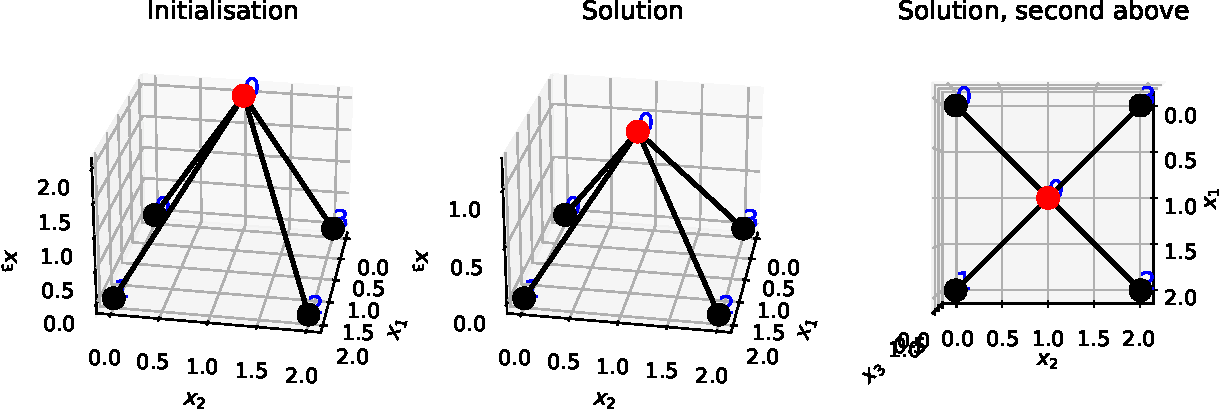
\includegraphics[width=\linewidth]{Bilder/localminpos.pdf}
\end{subfigure}%
\begin{subfigure}{.5\textwidth}
  \centering
  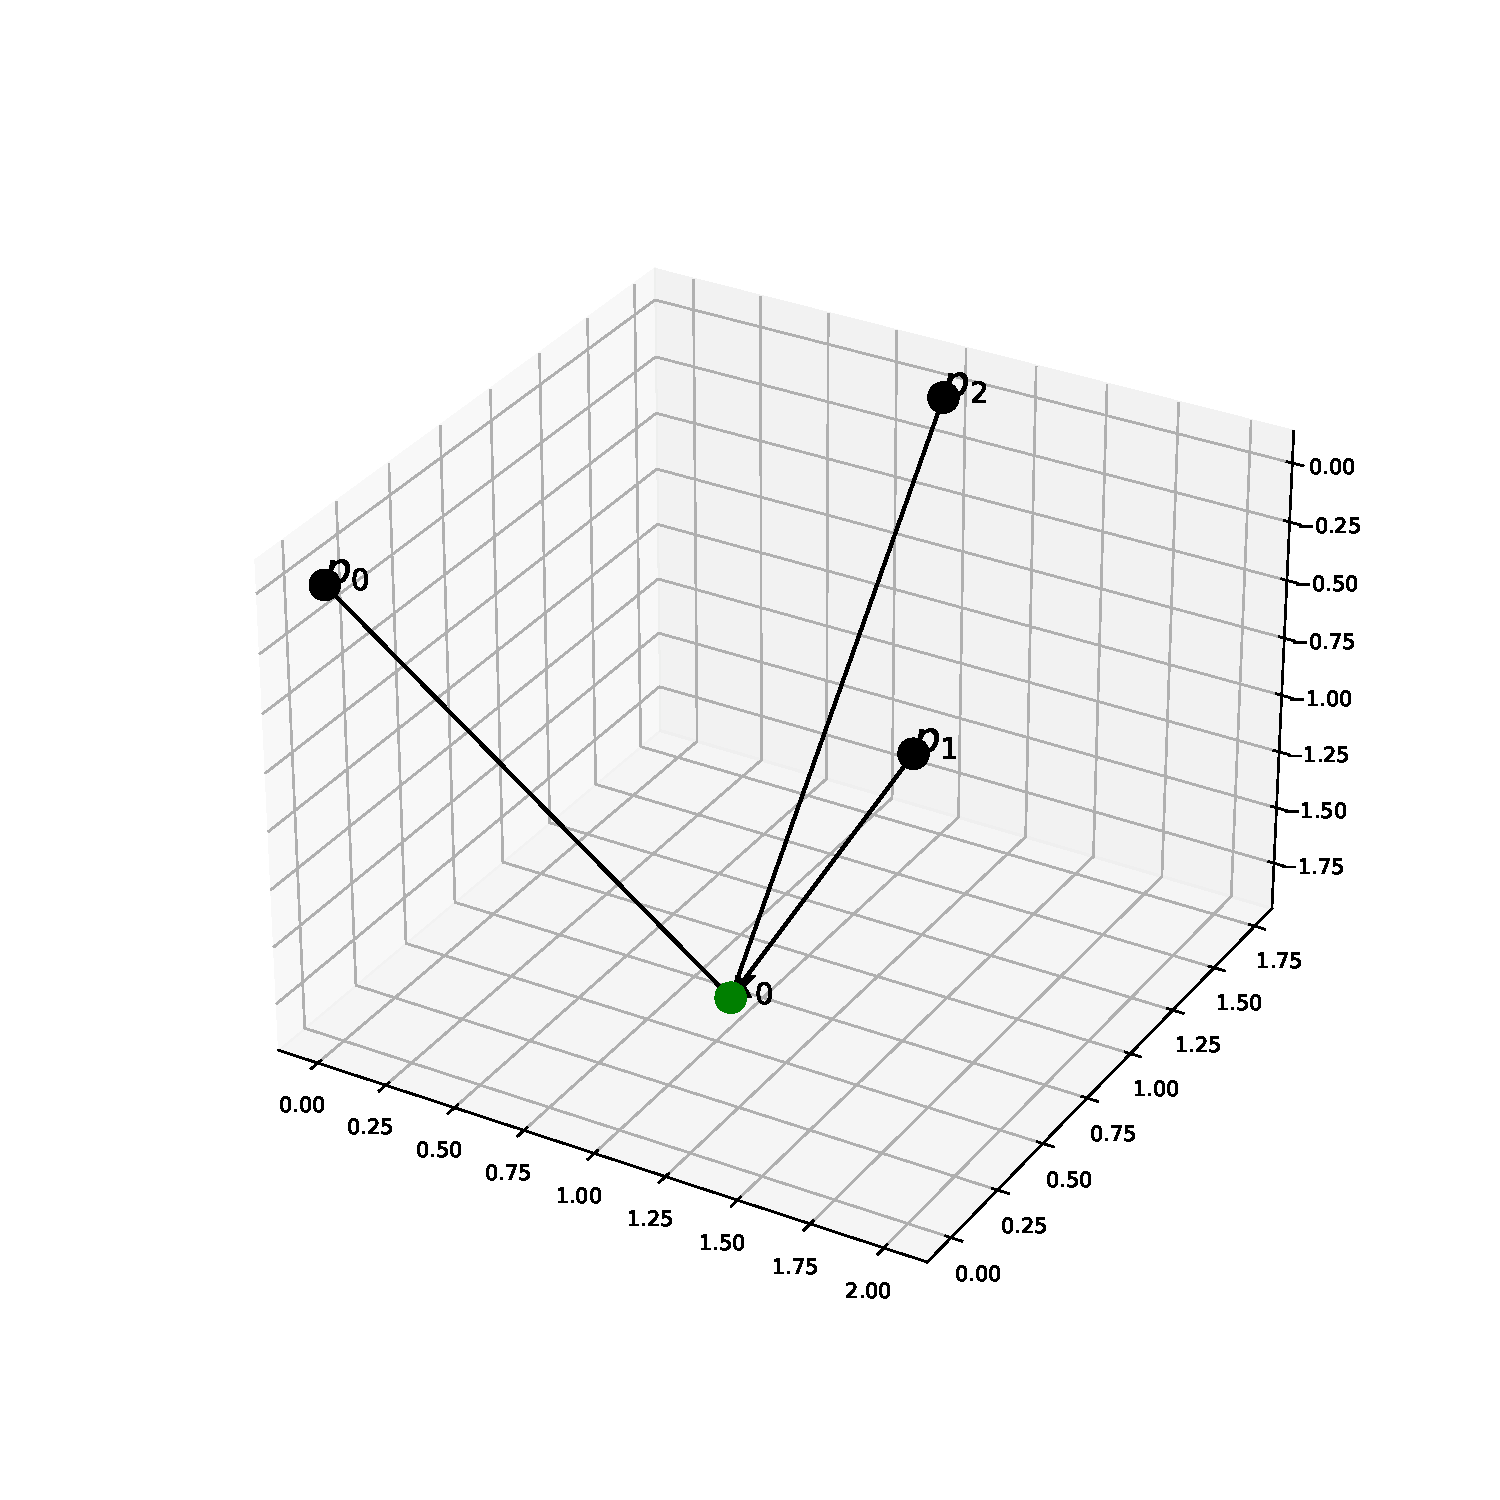
\includegraphics[width=1\linewidth]{Bilder/localminneg.pdf}
\end{subfigure}
\caption{Local optimizer to the left, global optimizer to the right. The free node $x^{(0)}$ placed above the $xy$-plane and is connected through bars to four fixed nodes. The position of $x^{(0)}$ will be determined by the equilibrium between external load, gravity, and elastic energy of the bar. However, if we initialize the free node below the $xy$-plane, we will reach a global minima. Notice that the $x_1$ and $y$-position is equal, only the $z$-component differs. Numerics will be discussed later in the paper. }
\label{fig:local_optimizer}
\end{figure}

\section{Tensegrity domes in constrained optimization}\label{sec:freestanding}
We will now consider the full problem \eqref{totalEnergy} with the constraints given by \eqref{z_positive}. As this is a constrained optimization problem, we define the Lagrangian \begin{equation}
    \mathcal{L}(X,\lambda) = E(X) - \sum_{i \in \ \mathcal{I}}\lambda_i c_i(X)
\end{equation}
Where $c_i(X) = x^{(i)}_3$. The first order optimality conditions for a given $(X^*,\lambda^*)$ are \begin{equation}
\begin{aligned}
       &\nabla_x \mathcal{L}(X,\lambda^*)=0\\ 
       &x^{*(i)}_3 \geq 0,\quad \lambda_i^* \geq 0 \quad \lambda_i^* x^{*(i)}_3 = 0,\quad i = 1,...,N\\
\end{aligned}
\end{equation}
As for LICQ we have 

\begin{align*}
    \nabla &c_1(X) = \bigg( \frac{\partial c_1}{\partial x^{(1)}},\frac{\partial c_1}{\partial x^{(2)}},...,\frac{\partial c_1}{\partial x^{(i)}},...,\frac{\partial c_1}{\partial x^{(N)}} \bigg) &&=\bigg( (0,0,1),(0,0,0),...,(0,0,0),...,(0,0,0) \bigg) \\
    % \vdots 
% \\
    \nabla &c_i(X) &&= \bigg( (0,0,0),(0,0,0),...,\underbrace{(0,0,1)}_{i^{\text{th}}\text{ term}},...,(0,0,0) \bigg)\\
    % \vdots \\
    \nabla &c_N(X) &&=\bigg( (0,0,0),(0,0,0),...,(0,0,0),...,(0,0,1) \bigg)
\end{align*}

It's clear that the inequality constraints $\{\nabla c_i(X),i=1,2,...,N\}$ are linearly independent as there are no vectors with non-zero terms in the same dimension. This means LICQ holds, and therefore the KKT conditions are neccesary, but they are not sufficient as our problem is not convex.

\subsection{Horizontal translational invariance}\label{sec:invariance}
Recall that a simultaneous shift of all nodes in any horizontal direction does not impact the total energy. For $\ece$ and $\ebe$, this is clear as the norm will be constant. As for $\ebg$ and $\ee$, these only depend on vertical shifts. When developing numerical methods, this can cause issues due to the non-uniqueness of solutions. The easiest workaround is to fix nodes, as discussed extensively in section \ref{subsec:fix} and \ref{subsec:fix2}.

